\chapter{Neural Ordinary Differential Equations}
\label{chapter:ode}

\section{Introduction}
\label{section:ode:introduction}

In recent years Residual Networks (ResNet) \citep{he2016deep} have brought a great success in Deep Learning and especially in computer vision. They have proven to be effective against the vanishing gradient and the degradation problems and have drastically eased the optimization of very deep neural networks. If we refer to the output vector of each layer as $ h_t $ where $ t $ stands for the layer, then Residual Networks can be mathematically described as:

\begin{equation}
    \label{equation:ode:resnet}
    h_{t+1} = h_{t} + f(h_{t}; \ \theta_{t})
\end{equation}

where $ t \in \{0, ..., T\} $, $ h_t \in R^D $ and $ \theta_t $ are the parameters of the \emph{t}-th layer. These iterative updates can be interpreted as an Euler discretization of a continuous transformation \citep{lu2017beyond, haber2017stable, ruthotto2018deep}.

Moreover, as we add more layers and take smaller steps, in the limit, we parameterize the continuous dynamics of the hidden state using an ordinary differential equation (ODE) \textcolor{red}{vo abbreviations ODE} specified by a neural network:

\begin{equation}
    \label{equation:ode:odes}
    \frac{d h(t)}{d t} = f(h(t), \ t; \ \theta )
\end{equation}

\citet{chen2018neural} introduced this concept as a new family of deep neural network models, where the neural network outputs the gradient of the hidden state with respect to the depth. Then, given an initial state and the differential equation parameterized by the neural network, the final state is obtained by solving an ODE. The analogy they make is the one that considers this family of models to be the continuous case of ResNets. Figure \ref{figure:ode:resnet_vs_ode}, depicts the similarities and differences between ResNets and neural networks based on ODEs. They call this family of models \emph{Neural ODEs} or \emph{ODENets}, and provide an open source framework implemented in PyTorch\footnote{https://github.com/rtqichen/torchdiffeq}.

\begin{figure}[ht]
      \centering
      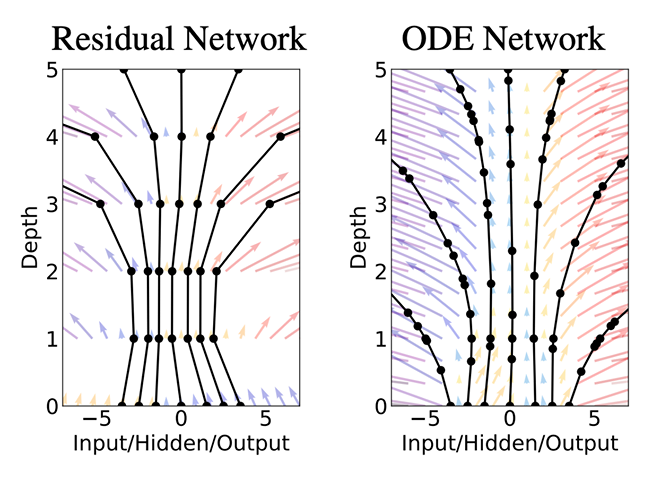
\includegraphics[width=0.7\columnwidth]{figures/resnet_vs_odes.png}
      \caption{\emph{Left}: A Residual network defines a discrete sequence of finite transformations. \emph{Right}: A ODE network defines a vector that continuously transforms the state \citep{chen2018neural}.}
      \label{figure:ode:resnet_vs_ode}
\end{figure}

In equation \ref{equation:ode:odes}, $ h(t) $ is the hidden state in the \emph{t}-th layer, and $ f $ can be any neural network parameterized by $ \theta $, with $ h(t) $ and $ t $ as inputs and the gradient of $ h(t) $ with respect to $ t $ as output. Furthermore, the final output of such a model can then be defined as:

\begin{align}
    z(t_1) & = z(t_0) + \int_{t_0}^{t_1} \frac{d h(t)}{d t} \\
    & = z(t_0) + \int_{t_0}^{t_1} f(h(t), \ t; \ \theta ) \\
    & = ODESolve(z(t_0), f, t_0, t_1)
\end{align}

According to the equation above, we can conclude that, $ f $ is learning a vector field, which is why Neural ODEs can potentially be seen as models with infinite amount of layers. To be specific, the number of layers is dynamically decided and delegated to the ODE solver. Furthermore, \citet{chen2018neural} developed their framework in way that any ODE solver can be used as a blackbox. This allows for more flexibility and decouples the framework from the ODE solver. General use ODENets are illustrated on Figure \ref{figure:ode:odenets_visualizations}.

\begin{center}
    \emph{\textcolor{red}{DIAGRAM OF WHAT ODENETS LOOK LIKE!}}
\end{center}

Defining neural network models in this fashion has several advantages \cite{chen2018neural}:

\begin{itemize}
    \item \textbf{Memory Efficiency.} In section \ref{section:ode:backpropagation} it is discussed how circumventing backpropagation through the operations of the ODE solver saves a lot of memory.
    \item \textbf{Adaptive Computation.} Nowadays, ODE solvers provide guarantees about the growth of the approximation error, monitor the error, and adapt their evaluation strategy on the fly to achieve the required level of accuracy. This allows for explicit control over the speed versus precision trade-off.
    \item \textbf{Parameter Efficiency.} In section 3 of their work, \citet{chen2018neural} show demonstrate how this family of models ties the weights of nearby layers, resulting in fewer parameters without the loss of performance.
    \item \textbf{Scalable and invertible normalizing flows.} In chapter \ref{chapter:cnf}, it is shown how one side effect of going in the continuous domain, allows for an easier and unrestricted use of normalizing flows. As a result, normalizing flows can be used for language modelling, as shown in chapter \ref{chapter:cnf_lm}.
    \item \textbf{Continuous time-series models.} RNNs are the de-facto architecture for time-series models. Unfortunately, they require that the observations are discretized and bound to specific emission intervals. On the other hand, continuously defined dynamics can naturally take care of observations that arrive at arbitrary times.
\end{itemize}

\section{Backpropagation through the ODE solver}
\label{section:ode:backpropagation}

An immediate question that rises, is how does one backpropagate through the ODE solver. In theory one can simply backpropagate through the operations of the solver, however, this has several drawbacks. First, some solvers, require solving a nonlinear optimization problem at every step. This can make direct backpropagation through the integrator difficult. Additionally, as mentioned in the previous section, ODENets can potentially have a very high number of layers. Backpropagating through such a large number of layers is inefficient from a memory point of view, as it would mean that all intermediate steps should be kept in memory until the backward pass is over. Therefore, what \citet{chen2018neural} propose, is to compute gradients by solving a second augmented ODE backwards in time. This method is called the \emph{adjoint sensitivity method} \citep{pontryagin2018mathematical} and is applicable to all ODE solvers. It scales linearly with problem size, has low memory cost, and allows for explicit control over numerical errors.

\begin{figure}[ht]
      \centering
      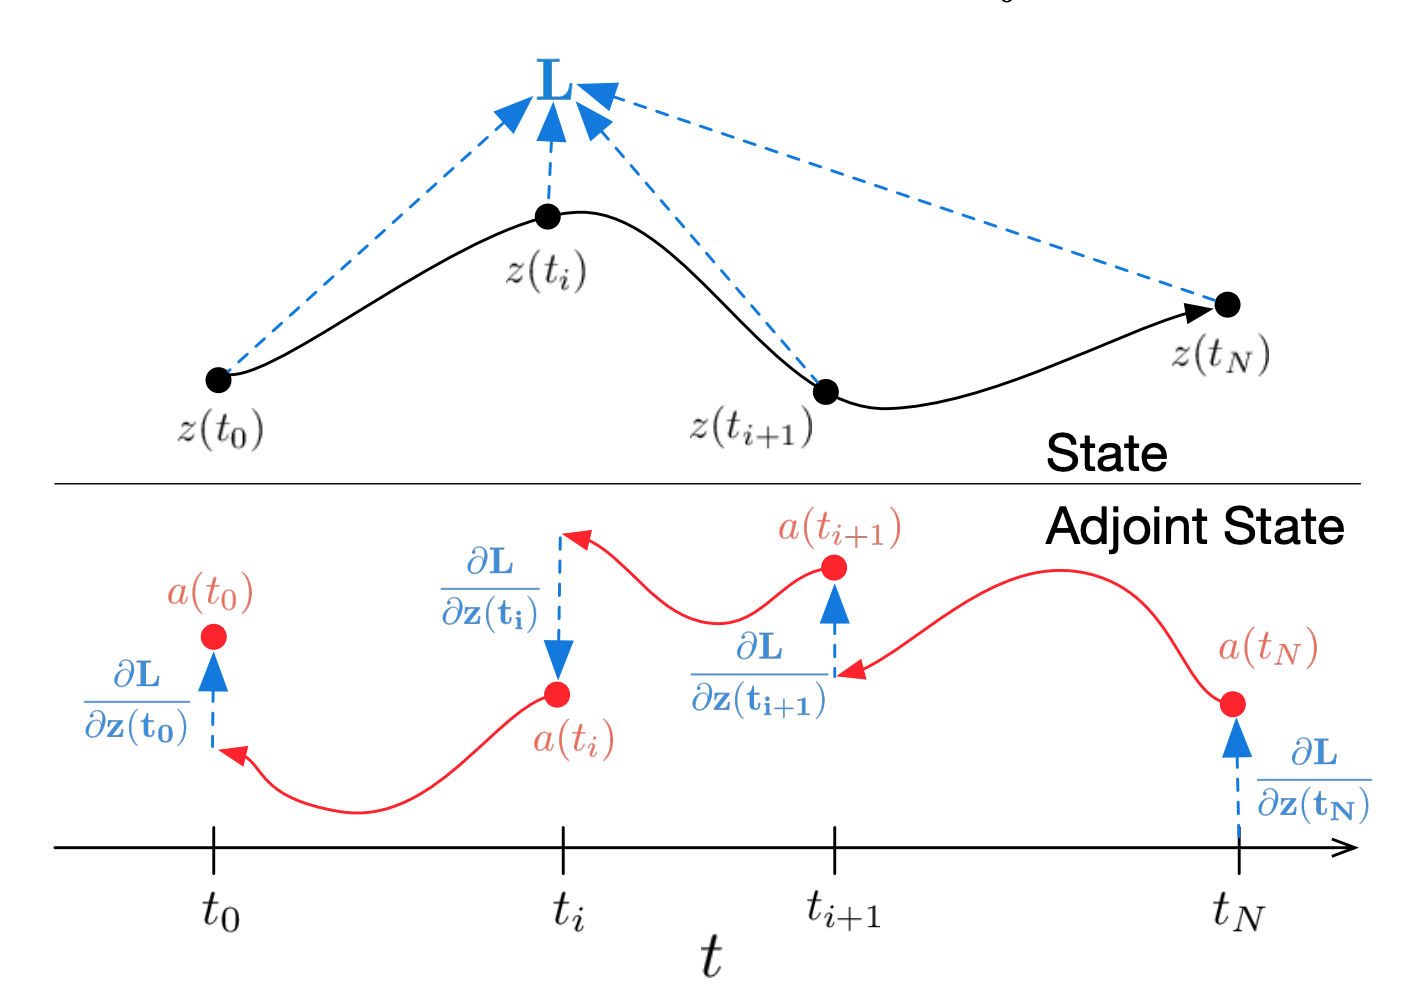
\includegraphics[width=\columnwidth]{figures/adjoint_method.png}
      \caption{Reverse-mode differentiation of an ODE solution. The adjoint sensitivity method solves an augmented ODE backwards in time. The red lines denote the sequence of separate ODE solves \cite{chen2018neural}.}
      \label{ode:adjoint}
\end{figure}

As shown in figure \ref{figure:ode:odenets_visualization}, we need to optimize a scalar valued loss function $ L $ whose input is the output of the ODE Solver.

\begin{equation}
    L(z(t_1)) = L \left( z(t_0) + \int_{t_0}^{t_1} f(h(t), \ t; \ \theta ) \right) = L(ODESolve(z(t_0), f, t_0, t_1))
\end{equation}

The parameters of the ODENet, are the parameters of the neural network $ f $ or $ \theta $, which is why we are interested in the derivative of the loss function with respect to $ \theta $. \citet{pontryagin2018mathematical} show that the derivative takes the form of another initial value problem

\begin{equation}
    \label{loss_derivative}
    \frac{dL}{d\theta} = - \int_{t_1}^{t_0} \left(\frac{\partial L}{\partial z(t)}\right)^T \frac{\partial f(z(t), \ t; \theta)}{\partial \theta}dt
\end{equation}

Where $ \nicefrac{\partial L}{\partial z(t)} $ is known as the \emph{adjoint state} of the ODE. \citet{chen2018neural} use one call to an ODE solver to get $ z(t_1) $ and then a second one to calculate the equation \ref{loss_derivative}. In cases where the loss depends not only on the final state $ z(t_1) $, but also on the intermediate states $ z(t) $, the reverse-mode derivative must be broken into a sequence of separate solves as shown on figure \ref{ode:adjoint}.

\section{Neural ODEs for Language Modelling}
\label{section:ode:ode_lms}

We can look at language modelling as a two step process. First, we encode the context into a hidden state vector, and then using the hidden state vector we generate a distribution over the vocabulary. The former is usually done by using a LSTM based RNN. Then, given the hidden state, a Softmax layer is used to obtain the probability distribution over the vocabulary. In section \ref{section:limitations:softmax_bottleneck}, it was discussed how having this Softmax layer, introduces a theoretical limitation on LMs, and in sections \ref{section:related_work:mos} and \ref{section:related_work:doc} was discussed how models like MoS \citep{yang2017breaking} and DoC \citep{takase2018direct} have tried to break it. In this section, I propose a simple model (figure \ref{figure:ode:ode_logits}) based on Neural ODEs, that does not suffer from the \emph{Softmax Bottleneck} problem.

\begin{center}
    \textcolor{red}{\emph{DIAGRAM OF WHAT THE MODEL LOOKS LIKE}}
\end{center}

Let $ V $ be the vocabulary, $ h $ be the hidden state, $ d $ be the hidden state dimensionality, $ L \in R^{d \times |V|} $ be the projection matrix (if weights are tied this is also the embedding matrix), and $ y^* \in R^{|V|} $ be a one hot encoded ground truth vector. Then:

\begin{align*}
    l(t_0) &= L^T h, \ l \in R^{|V|} \\
    l(t_1) &= node(l(t_0), \ f) \\
    y &= Softmax(l(t_1))
\end{align*}

Where $ node $ is a NeuralODE block and is defined as:

\begin{displaymath}
    node(l(t_0), \ f) = l(t_0) + \int_{t_0}^{t_1} f(l(t), \ t) dt    
\end{displaymath}

and $ f $ is a neural network parametrizing the gradient of the logits $ l $ with respect to time or in this case depth, and can be an arbitrary neural network architecture. One possibility is to define it as:

\begin{displaymath}
    f(l, t) = H_f ReLU(W_f^T l), \ W_f, H_f \in R^{|V| \times |V|}    
\end{displaymath}

One problem with this approach lies in the $ W_f, H_f \in R^{ |V| \times |V| } $ matrices. As the vocabulary can often be in the tens of thousands, this highly increases both the memory and the time complexity of the overall model. However, this problem can be solved by using a bottleneck:

\begin{displaymath}
    f(l, t) = H_f ReLU(W_f^T l), \ W_f, H_f \in R^{|V| \times k}    
\end{displaymath}

Where $ k $ is the dimensionality of the bottleneck and is usually in the low hundreds.

In the simplest form of $ f $, $ t $ can be ignored. This is the same as saying that the gradient does not depend on it and we have a constant vector field as we move through time. Other possibilities are to concatenate it to the input or use it in a conjunction with Hypernetworks \citep{ha2016hypernetworks} to generate $ W_f $ and $ H_f $ based on $ t $. Both approaches are suggested in \citet{chen2018neural} and \citet{grathwohl2018ffjord}. Finally, we can use Cross Entropy as a loss function:

\begin{displaymath}
    CE(y^*, y) = - \sum_{i=1}^{|V|} y^*_i \log y_i
\end{displaymath}

And as $ y^* $ is one-hot encoded ground truth vector, this boils down to:

\begin{displaymath}
    CE(y^*, y) = - \log y_{i^*}
\end{displaymath}

Where $ i^* $ is the single component of $ y^* $ that is not zero.

The main idea behind this approach is to solve the softmax bottleneck by applying non-linear transformations on the logits, similar to what is done in \citep{ganea2019breaking}. The difference between the two approaches lies in the nature of the non-linearities applied. \citet{ganea2019breaking} apply monotonic pointwise non-linearities, and here we use a NeuralODE.
